\documentclass[11pt]{scrartcl}

\usepackage[utf8]{inputenc}
\usepackage[spanish]{babel}

\usepackage{parskip}
\usepackage{graphicx}

\title{Taller de programación III (75.61)\\[0.2em]\Large{Facultad de Ingeniería de la UBA}\\[1em]}
\subtitle{\huge{TP1: Contador de visitas y pruebas de carga\\[0.2em]Documento de diseño}}
\author{Adrián Barreal\\\small{Segundo cuatrimestre 2021}}
\date{}

\begin{document}
\maketitle
\tableofcontents
\newpage

%========================================================================
%========================================================================
\section{Introducción}

Este documento detalla el diseño y arquitectura del sistema desarrollado para un sitio 
institucional con requisitos de escalabilidad y tolerancia a fallos. El sistema fue diseñado en base
a tecnologías provistas por Google Cloud, donde el sistema sería eventualmente desplegado.

El documento se estructura acorde al modelo C4 de visualización de software.
En la sección \ref{sec:system} se describe el sistema de software en su contexto;
en la sección \ref{sec:containers} se describen los contenedores, 
elementos ejecutables y autónomos que hacen al sistema;
en la sección \ref{sec:components} se describen los componentes que hacen a cada contenedor;
y en la sección \ref{sec:code} se dan detalles adicionales sobre el código de cada componente.

%========================================================================
%========================================================================
\section{Contexto del sistema de software}\label{sec:system}

El sistema consiste esencialmente en una aplicación web. El sistema que da soporte a esta aplicación debe cumplir con los requisitos de escalabilidad y tolerancia a fallos. Para cumplir con dichos requisitos se hace uso de las tecnologías provistas por Google Cloud Platform. El resultado es un sistema como se esquematiza en la figura \ref{fig:system}. En todos los diagramas la orientación de las flechas indica esencialmente quién invoca a quién, o quién le envía pedidos o inicia la interacción con quién, salvo que se indique lo contrario.

\begin{figure}
\centering
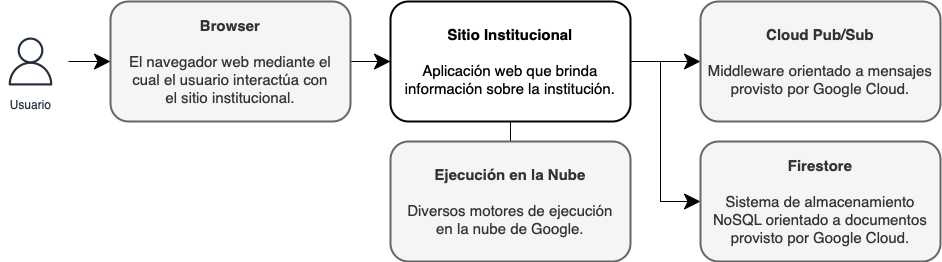
\includegraphics[scale=0.44]{img/context}
\caption{Diagrama de contexto del sistema a implementar.}
\label{fig:system}
\end{figure}

El usuario interactúa con el sistema a través de su navegador. El sistema hace uso de la base de datos Firestore orientada a documentos para almacenar datos en forma persistente. Para cumplir con los requisitos de escalabilidad y tolerancia a fallos se utiliza también Cloud Pub/Sub para permitir el despacho de tareas asincrónicas con consistencia eventual.

%========================================================================
%========================================================================
\section{Contenedores}\label{sec:containers}

\subsection{Elementos autónomos y ejecutables}

Los elementos autónomos y ejecutables que hacen al sistema son los que se esquematizan en la figura \ref{fig:containers}.

\begin{figure}
\centering
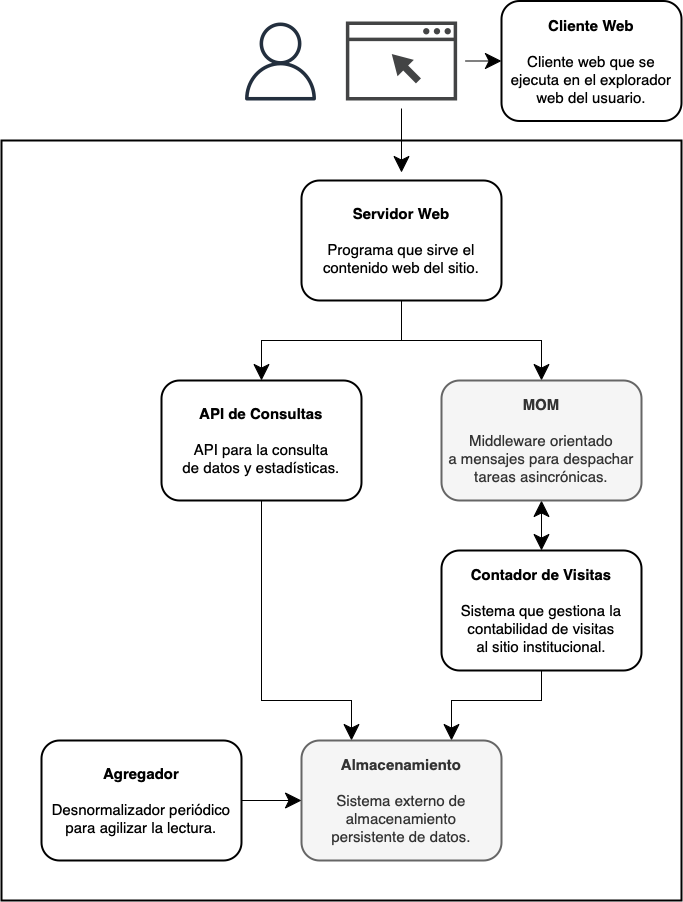
\includegraphics[scale=0.6]{img/containers}
\caption{Diagrama de contenedores del sistema a implementar.}
\label{fig:containers}
\end{figure}

\begin{itemize}
\item \textbf{El cliente web}. Este elemento se ejecuta en el navegador del usuario. No se comunica directamente con el resto del sistema, pero implementa funcionalidad del lado del cliente relacionada a la presentación de contenido.
\item \textbf{El servidor web principal}. Es el servidor que se encarga de servir el contenido web HTML propiamente dicho, y también otros recursos estáticos como imágenes, archivos CSS y código JavaScript.
\item \textbf{La API de consultas}. Es un subsistema interno que otras aplicaciones pueden consumir y encapsula el acceso de lectura al sistema de almacenamiento, y eventualmente también escrituras que deban ser fuertemente consistentes.
\item \textbf{El middleware orientado a mensajes}. En principio provisto externamente. Se utiliza concretamente Cloud Pub/Sub, como se adelantó en la sección \ref{sec:system}. Cualquier middleware orientado a mensajes debería resultar adecuado, no obstante, mientras pueda soportar la carga esperada para la aplicación.
\item \textbf{El contador de visitas}. Es el elemento encargado de recibir y procesar tareas de contabilidad de visitas despachadas a través del middleware orientado a mensajes.
\item \textbf{El agregador}. Tiene la tarea de recolectar datos previamente escritos al sistema de almacenamiento y producir resultados agregados a una cadencia reducida. Esto tiene el objetivo de reducir el tiempo de procesamiento globalmente destinado a calcular estadísticas, y también a reducir la cantidad de consultas al sistema de almacenamiento con el objetivo de minimizar el costo por lectura de datos.
\item \textbf{El sistema de almacenamiento persistente}. Provisto externamente. Se utiliza concretamente la base de datos no relacional Firestore de Google Cloud. Se adoptó esta base por los requisitos de escalabilidad. Concretamente, para contabilizar las visitas se adoptó un sistema de sharding que será explicado en breve, y cualquier reemplazo debería soportar funcionalidad similar.
\end{itemize}

\subsection{Escalabilidad y tolerancia a fallos}

\begin{figure}
\centering
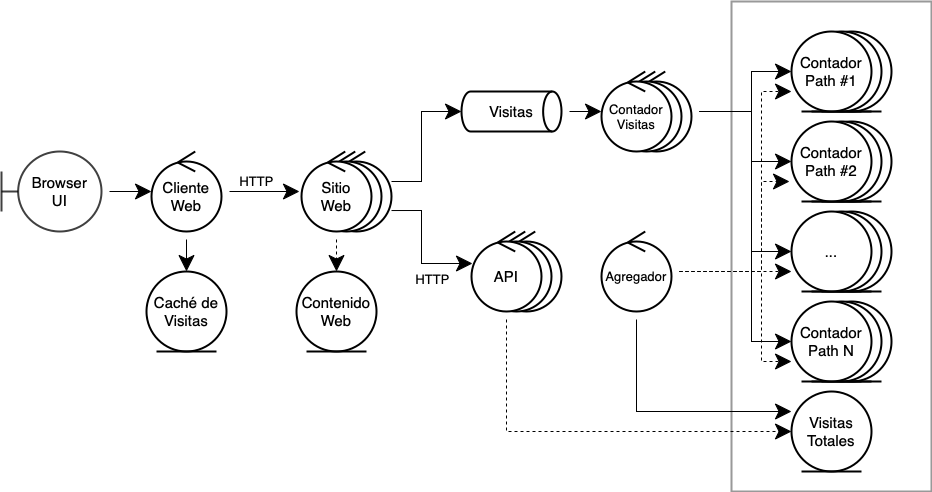
\includegraphics[scale=0.45]{img/robustness}
\caption{Diagrama de robustéz del sistema a implementar. Las flechas rayadas indican lectura.}
\label{fig:robustness}
\end{figure}

La figura \ref{fig:robustness} es un diagrama de robustéz que esquematiza los elementos del sistema y su capacidad de escalar. El sistema soporta escalamiento horizontal debido en principio a las siguientes decisiones de diseño:

\begin{itemize}
\item Los elementos de cómputo cuya carga se espera que sea dinámica se ejecutan en los motores de Google Cloud que cuentan inherentemente con capacidad de autoescalamiento. Se hace uso de Cloud Run y Cloud Functions para desplegar una cantidad dinámica de instancias, cuya cota superior es configurable para cada elemento. El sistema de la nube se encarga también de mantener una cantidad mínima de instancias vivas si es posible y necesario, ahorrando en principio la necesidad de implementar un sistema de monitoreo sofisticado.
\item Firestore sufre de notables limitaciones en lo que respecta a escrituras concurrentes. Para mitigar los riesgos de la degradación de rendimiento por problemas de contención se implementó un mecanismo de contabilidad de visitas particionado en múltiples shards. Existen múltiples contadores (uno para cada página de la que se quiera contabilizar visitas) y cada contador está dividido a su vez en múltiples shards (sub-contadores). Aumentar un contador implica entonces seleccionar uno de sus shards según algún criterio (e.g. aleatorio uniforme) y aumentar el entero asociado a ese shard particular. La cantidad de shards por contador es configurable y puede aumentar y disminuir durante el tiempo de vida del sistema sin causar corrupción de datos.
\item Del ítem anterior se desprende que leer un contador implica sumar los valores almacenados en cada uno de sus shards. Visto que el contador debe ser leído en cada acceso se implementó un mecanismo de agregación que calcula la suma de todos los shards de todos los contadores a intervalos periódicos y produce un resultado que puede ser consumido con una sola lectura. Esto ahorra por un lado en tiempo de cómputo, pero también en solicitudes de lectura a Firestore que tienen individualmente un costo económico asociado.
\item La utilización del agregador implica inevitablemente consistencia eventual.  Para agilizar el servicio del contenido web, conseguir un mejor desacople, y ganar en tolerancia a fallos, se utilizó Pub/Sub como middleware orientado a mensajes para gestionar las escrituras a Firestore (en principio solo los contadores) en forma asincrónica.
\item La consistencia eventual puede producir resultados poco prolijos del lado del cliente. El problema más obvio sería que el contador permanezca constante incluso ante los propios cambios de página del usuario. Para dar la ilusión de consistencia fuerte en el contador se puede implementar un script en el navegador web que utiliza un caché local en session storage. El script mantiene su propio contador de visitas que aumenta cada vez que el usuario cambia de página si servidor todavía no actualizó su cuenta. El contador local se restablece automáticamente en cero cuando el script detecta que el servidor proveyó una cuenta actualizada y utiliza esta última como nueva fuente de verdad. El resultado es una experiencia más natural para el usuario.
\end{itemize}

\subsection{Despliegue}

El despliegue en Google Cloud Platform se esquematiza en la figura \ref{fig:deployment}.  Todos los elementos han de ser desarrollados en forma contenedorizada simplificar el despliegue y la gestión.

\begin{figure}
\centering
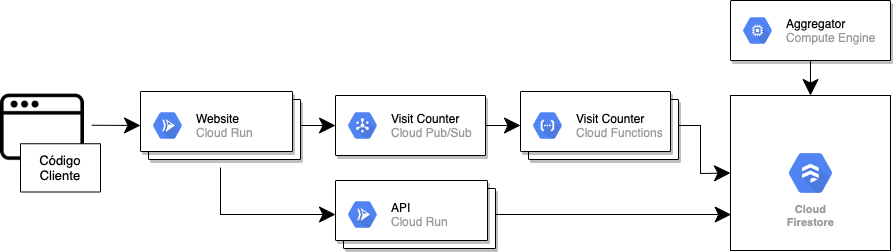
\includegraphics[scale=0.48]{img/deployment}
\caption{Despliegue en Google Cloud Platform.}
\label{fig:deployment}
\end{figure}

Tanto el sitio web como la API reciben tráfico dinámico y deben ser escalables, con lo cual han de ser desplegados en Cloud Run. El componente que contabiliza las visitas puede ser más fácilmente implementado como una Cloud Function, por otro lado, con lo cual es conveniente desplegarlo de ese modo. El agregador, como se comentó, no requiere escalar horizontalmente mientras pueda realizar su tarea de agregación en un tiempo razonable, con lo cual puede ser desplegado en Compute Engine usando una máquina virtual con Container OS, un mecanismo simplificado que provee Google para desplegar contenedores. El funcionamiento del sistema requiere también la definición de un tópico de Pub/Sub, cuyo nombre debe ser configurado en los elementos que interactúan con el middleware. El cliente web, por otro lado, será provisto por el servidor web al navegador.

\subsection{Parámetros de despliegue}

Los listados a continuación son parámetros configurables al momento de realizar el despliegue del sistema. Se proponen adicionalmente algunos valores iniciales para alimentar pruebas que puedan servir para determinar una configuración más adecuada.

\begin{itemize}
\item Cantidad máxima de instancias del contenedor web en Cloud Run: 2.
\item Cantidad máxima de instancias de la API en Cloud Run: 2.
\item Cantidad máxima de instancias del contador de visitas en Cloud Functions: 2.
\item Cantidad de shards por contador en Firestore: 100.
\item Recursos por instancia: 1 CPU y 1 GB de memoria.
\end{itemize}

%========================================================================
%========================================================================
\section{Componentes}\label{sec:components}

\subsection{Sitio web}

\begin{figure}
\begin{center}
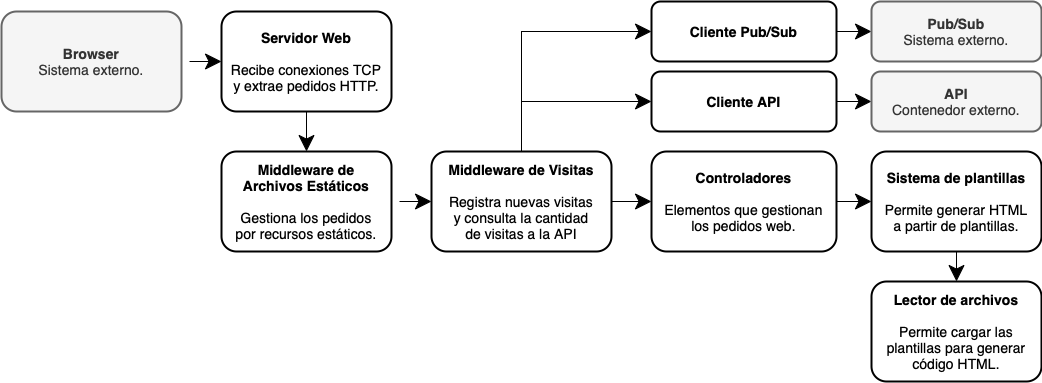
\includegraphics[width=\linewidth]{img/website-component}
\end{center}
\caption{Componentes que hacen al sitio web.}
\label{fig:website}
\end{figure}

Los componentes que hacen al sitio web se muestran en la figura \ref{fig:website}. Existe en principio un componente que implementa el servidor web en sí, en general provisto externamente (e.g. Express para Node.js). Existe luego una cadena de filtros (o middlewares, como se los suele llamar). El primero sirve archivos estáticos bajo la ruta \texttt{\textbackslash{}static}; esto incluye archivos de imágenes, hojas de estilos y scripts. El segundo middleware se encarga de contabilizar visitas y recuperar la cuenta más reciente de visitas para aquellas rutas que no correspondan a archivos estáticos (los endpoints principales de la aplicación). En principio este middleware hace uso de los clientes de PubSub y de la API, aunque puede eventualmente refactorizarse e implementar una capa de servicios para encapsular el uso de estos elementos. Finalmente están los controladores que generan el contenido HTML en base a plantillas. Existen controladores para los siguientes endpoints, correspondientes al contenido previsto del sitio:

\begin{itemize}
\item \texttt{/home}
\item \texttt{/jobs}
\item \texttt{/about}
\item \texttt{/about/offices}
\item \texttt{/about/legals}
\end{itemize}

Existen luego rutas adicionales para archivos estáticos:

\begin{itemize}
\item \texttt{/static/css}
\item \texttt{/static/img}
\item \texttt{/static/js}
\end{itemize}

Estas últimas son gestionadas por el middleware de archivos estáticos, aunque eventualmente pueden ser delegadas a un nginx, a Cloud Storage, o a algún otro sistema optimizado para servirlos, mediante la incorporación de un proxy reverso.

\subsection{API web}

\begin{figure}
\begin{center}
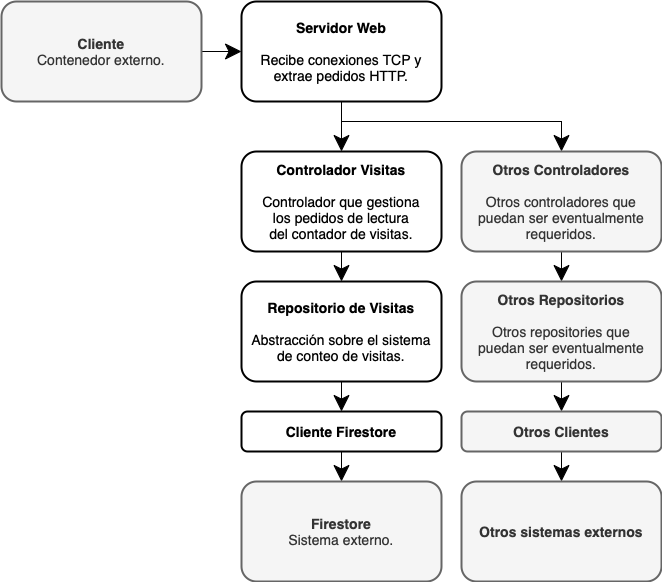
\includegraphics[width=\linewidth]{img/api-component}
\end{center}
\caption{Componentes que hacen a la API web.}
\label{fig:api}
\end{figure}

Los componentes que hacen a la API web se esquematizan en la figura \ref{fig:api}. La arquitectura es similar a la del sitio web, aunque la API no tiene la responsabilidad de servir contenido web sino más bien de responder a pedidos HTTP con respuestas en formato JSON. Se requiere en principio un único controlador para dar acceso al contador de visitas a las aplicaciones que lo requieran. Para encapsular el acceso al contador existe una abstracción tipo repositorio que internamente utiliza el cliente de Firestore para leer el resultado que periódicamente actualiza el agregador. No se adoptó una capa de servicios debido a la funcionalidad limitada que fue en principio requerida. Implementar dicha capa sería adecuado si la funcionalidad de la API creciera. La versión actual expone solo el endpoint \texttt{/api/visits/total} que permite obtener el total de visitas registradas en el sitio.

\newpage
\subsection{Contador de visitas}

\begin{figure}
\begin{center}
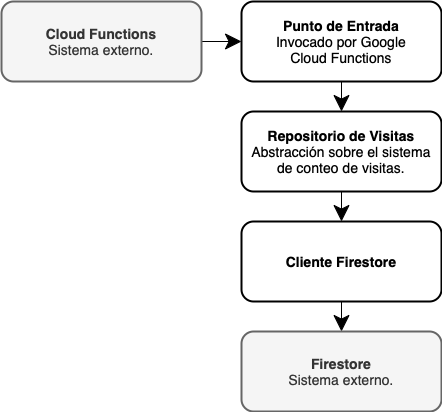
\includegraphics[scale=0.7]{img/visitcount}
\end{center}
\caption{Componentes que hacen al contador de visitas.}
\label{fig:visitcount}
\end{figure}

Los componentes que hacen al contador de visitas se esquematizan en la figura \ref{fig:visitcount}. Se trata de una Cloud Function con responsabilidad acotada. Lo único que hace es recibir un mensaje por Pub/Sub que indica que una visita ha de ser contabilizada. Un ejemplo de mensaje se muestra a continuación:
 \begin{verbatim}
{
	"path": "/home"
}
\end{verbatim}

Se trata de un objeto JSON que indica la ruta del recurso para hay que sumar una visita.

\textbf{Limitación actual}: el contador de visitas no cuenta con un filtro de duplicados. De resultar necesario se puede implementar haciendo uso de Firestore. Esto tendría un impacto en el rendimiento, no obstante, y también en los costos, ya que implicaría al menos una escritura por visita al sitio y una cantidad de lecturas dependiente de los detalles concretos de la implementación. Esto tendría un costo económico adicional ya que las operaciones en Firestore tienen costo individual, y hay que contemplar los ya mencionados problemas de contención.

\subsection{Agregador}

\begin{figure}
\begin{center}
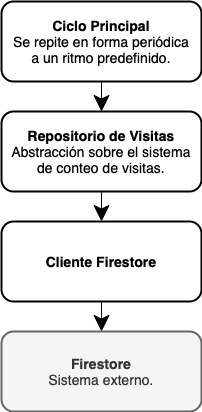
\includegraphics[scale=0.7]{img/aggregator}
\end{center}
\caption{Componentes que hacen al agregador.}
\label{fig:aggregator}
\end{figure}

Los componentes que hacen al agregador se esquematizan en la figura \ref{fig:aggregator}. Se trata simplemente de un worker que periódicamente ejecuta una tarea de agregación de contadores como se describió previamente. Dicha tarea consiste en leer todos los shards de todos los contadores de visitas en Firestore, calcular la suma, y guardarla en un contador individual que agrega los resultados. Este contador puede ser leído en una sola operación. La frecuencia de agregación es configurable.

El comportamiento del agregador se describe en el diagrama de actividades de la figura \ref{fig:aggregator-activity}. Se utiliza el iterador provisto por la biblioteca de Firestore para iterar por cada uno de los contadores, acumulándolos en un único contador que será escrito a una única entidad.

\begin{figure}
\begin{center}
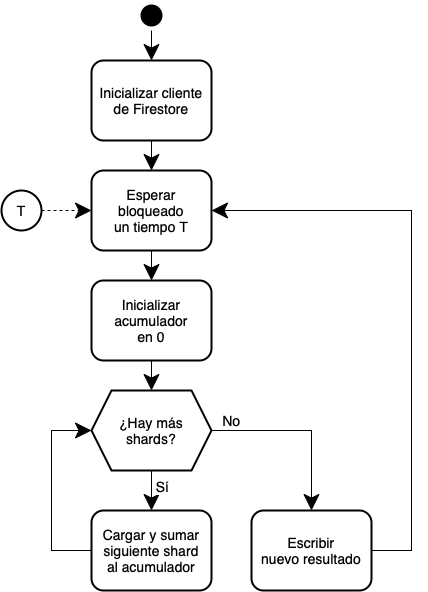
\includegraphics[scale=0.7]{img/aggregator-activity}
\end{center}
\caption{Diagrama de actividades del agregador. Suma todos los shards de todos los contadores a un intervalo configurable $T$.}
\label{fig:aggregator-activity}
\end{figure}

%========================================================================
%========================================================================
\section{Código}\label{sec:code}

\subsection{Sitio web}

\begin{figure}
\begin{center}
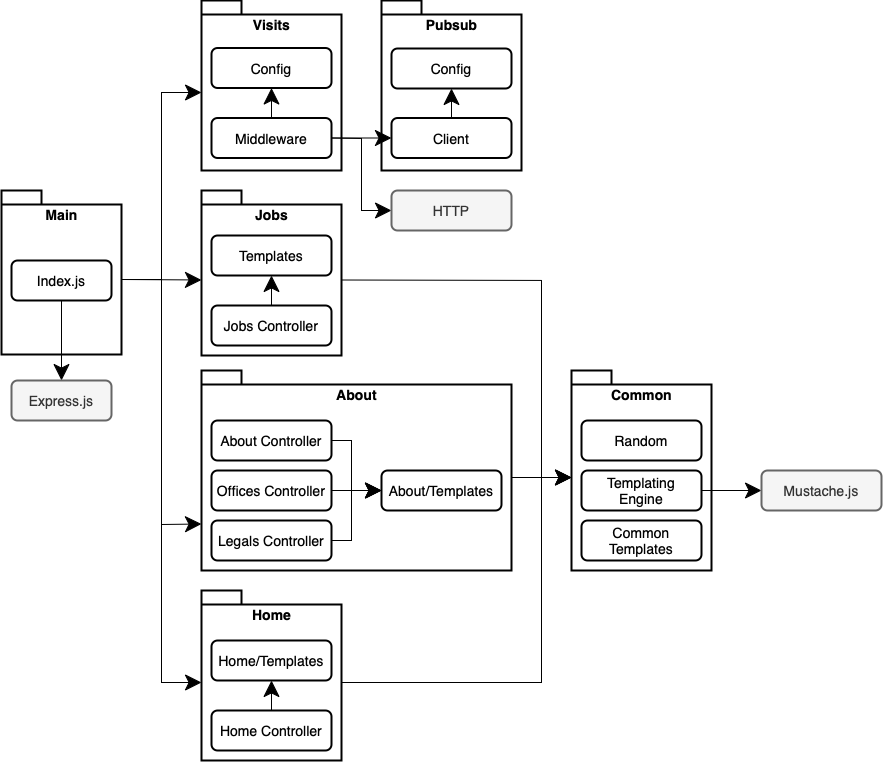
\includegraphics[width=\linewidth]{img/website-packages}
\end{center}
\caption{Diagrama de paquetes de la aplicación del sitio web.}
\label{fig:website-packages}
\end{figure}

En la figura \ref{fig:website-packages} se ve un diagrama de los paquetes que hacen a la aplicación del sitio web. Se implementó un sistema básico de generación de contenido HTML en base a plantillas usando \texttt{Mustache.js}, utilizado por todos los controladores. Cada sección del sitio está en su propio paquete y tiene su propio conjunto de plantillas. La plantilla del layout común está definida también en el paquete Common.

Para implementar el conteo de visitas se definió un middleware de Express, el servidor web utilizado. El middleware utiliza el cliente definido en el paquete PubSub para publicar mensajes al servicio, y el cliente HTTP para hacer pedidos a la API. De implementarse endpoints adicionales sería adecuado encapsular el acceso a la API en su propio cliente.

Para configurar la aplicación se utilizaron variables de entorno. El acceso a estas variables se encapsuló en módulos de configuración dentro de cada paquete. De requerirse mecanismos de configuración más sofisticados, estos podrían ser implementados en el paquete Common y ser consumidos por los módulos de configuración sin modificar su interfaz.

\subsection{Restantes componentes}

La API, el contador de visitas y el agregador están escritos en Go y tienen arquitecturas relativamente simples debido a la funcionalidad reducida que implementan. El conjunto de los paquetes que hacen a las tres aplicaciones se muestra en la figura \ref{fig:gomodules-packages}. 

El paquete Storage es compartido e implementa un repositorio que encapsula el acceso a Firestore para cuestiones relacionadas a la contabilidad de visitas. El contador de visitas desplegado como una Cloud Function lo utiliza para contar nuevas visitas, el agregador lo utiliza para ejecutar el procedimiento de agregación de visitas, y la API lo utiliza para obtener el último valor del contador registrado por el agregador. La API hace adicionalmente uso del servidor web Gin para recibir y despachar los pedidos web al controlador o a los eventuales controladores.

\begin{figure}
\begin{center}
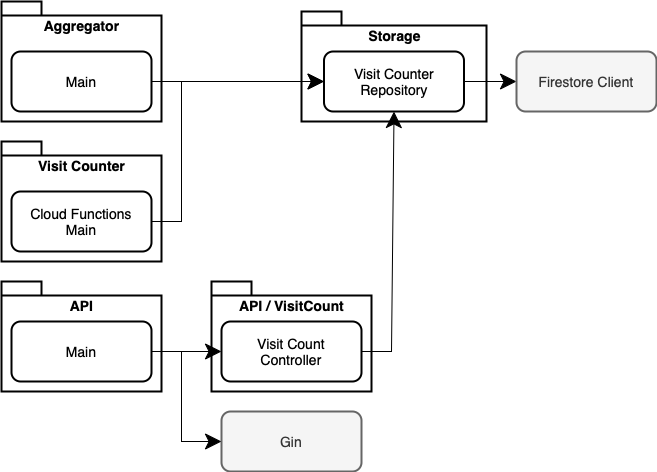
\includegraphics[width=\linewidth]{img/gomodules}
\end{center}
\caption{Diagrama de paquetes de los componentes de software escritos en Go.}
\label{fig:gomodules-packages}
\end{figure}

\end{document}